\chapter{Design and Development: Sensors for Data Collection} 
\label{sensors}

The {\bf Sensors} in this report refer to the separate sensors connected to the body of the patient which collects raw measurements of vital sign paramaters, conditions the data so that it is suitable for analogue to digital conversion, and converts the data into a digital signal that can be interpreted by the platform ({\bf Terminals}). \\

The sensors used in this project are enumerated as follows with the respective vital sign parameter measured: 

\begin{enumerate}
	\item ECG - AD8232 Heart Rate Monitor 
	\item PPG - GC1 PPG Sensor
	\item EEG - Neurosky TGAM Module
	\item Blood Temperature - Thermistor in Phase Shift Oscillator Configuration
\end{enumerate}

The following sections below further discusses the reason behind the choices made for the individual sensors, the mechanism of operation, and how it interfaces with the entire system. 

\section{ECG}
\label{ecgdevices}

The ECG front end design consists of a number of parts. 

The typical range of an ECG signal lies between $0.01\sim 300Hz$ and $0.05\sim 3mV$ in terms of frequency and amplitude respectively \cite{nisignalamplitude}. The voltages sampled from the surface of the skin through electrodes are too miniscule to be directly plotted and displayed. In addition, there are multiple frequencies which are of interest in ECG signals but the raw measurements will contain unwanted signal artifacts from other sources. Hence, it is necessary to amplify and filter the signal before any analysis or visualisation is performed.  

In 1997, Strohmenger \cite{strohmenger1997analysis} did an analysis of ventricular fibrillation ECG signal amplitude and frequency parameters for both successful and unsuccesful cardiac arrest countershocks. In this paper, the frequency range and amplitude range of both cases corroborates with the typical values stated above.  



\subsection{AD8232 IC ECG Sensor}

In this project, in line with the aim of producing a system that is a working proof of concept, a simplified version of the ECG is used. The AD8232 IC from Analog Digital was used \cite{ad8232datasheet}. 

\begin{figure}[H]
	\centering
	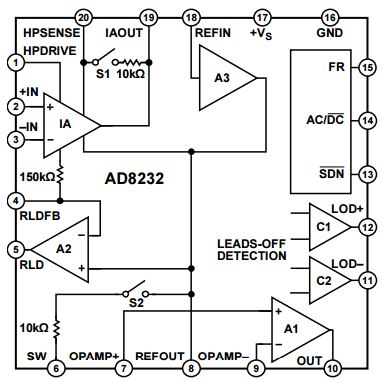
\includegraphics[width=0.4\linewidth]{ad8232funcdiagram.jpg}
	\caption{AD8232 Functional Block Diagram \cite{ad8232datasheet}}
	\label{ad8232functional}
\end{figure}

\subsubsection{Front End}

The Analog Devices AD8232 was used to implement the ECG part of this project. The AD8232 is "an integrated signal conditioning block for ECG", "designed to extract, amplify, and filter small biopotential signals" \cite{ad8232datasheet}. The functional block diagram is included above in Figure \ref{ad8232functional}. 

%\begin{figure}[H]
%	\centering
%	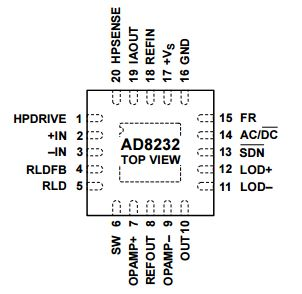
\includegraphics[width=0.4\linewidth]{ad8232pin.jpg}
%	\caption{AD8232 Pin Configuration \cite{ad8232datasheet}}
%	\label{ad8232pin}
%\end{figure}

\subsubsection*{Theory of Operation of the AD8232}

\begin{figure}[H]
	\centering
	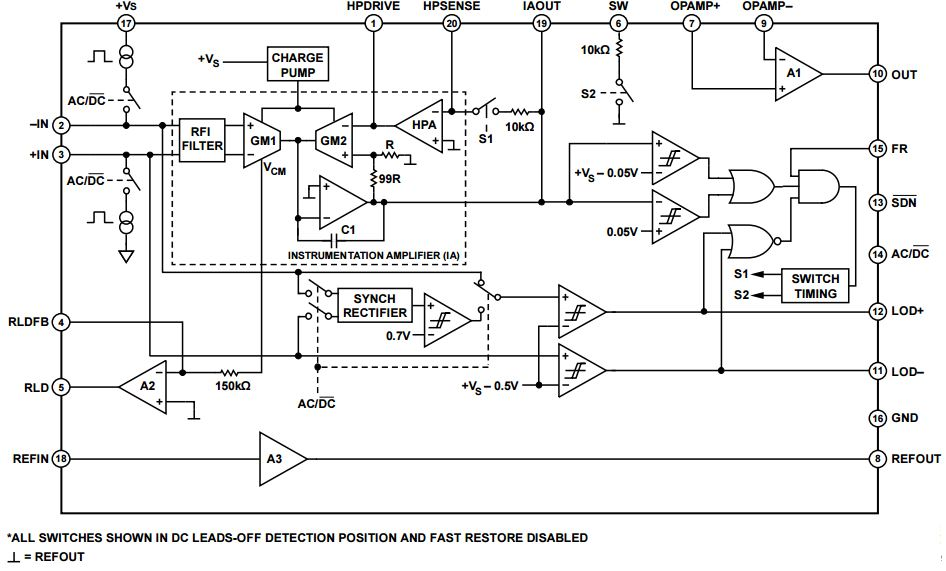
\includegraphics[width=\linewidth]{ad8232schematic.jpg}
	\caption{AD8232 Simplified Schematic Diagram \cite{ad8232datasheet}}
	\label{ad8232schematic}
\end{figure}

Figure \ref{ad8232schematic} above shows the architectural overview of the AD8232 chip from Analog Devices used for the "front end signal conditioning of cardiac biopotentials" \cite{ad8232datasheet} and is comprised of the following components: 

\begin{itemize}
	\item Specialized instrumentation amplifier (IA) - Amplifies ECG signals 
	\item Operational amplifier (A1) - For low pass filtering and supplying extra gain 
	\item Right leg drive amplifier (A2) - Improves common-mode signal rejection by inverting the signal 
	\item Midsupply reference buffer (A3) - Provides a reference signal for the IA by creating a virtual ground between the supply voltage and system ground 
	\item Leads off detection circuitry - Senses and indicates if the electrodes have been disconnected
	\item Automatic fast restore circuit - Decrease settling time of the ECG signal for a quicker response 
\end{itemize} 

\subsubsection*{AD8232 IC Cardiac Monitor Circuit Configuration}

The datasheet for the AD8232 provided by Analog Devices supplies a typical circuit setup and configuration for a cardiac monitoring as seen in the schematic diagram in Figure \ref{ad8232cardiacconfig} below \cite{ad8232datasheet}. A printed circuit board with this configuration could have been assembled and constructed using Altium Designer but due to time and cost constraints, an exact implementation of this circuit (with additional headers, an LED indicator, and a 3.5mm jack for biomedical pad connection) from SparkFun Electronics was used instead \cite{ad8232}.   

\begin{figure}[H]
	\centering
	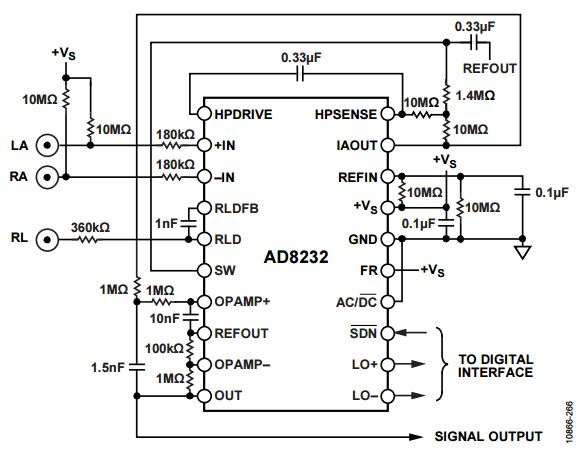
\includegraphics[width=0.6\linewidth]{ad8232cardiacconfig.jpg}
	\caption{Circuit Configuration for ECG Waveform Monitoring using the AD8232 \cite{ad8232datasheet}}
	\label{ad8232cardiacconfig}
\end{figure}
 
The schematic of the actual schematic capture of the AD8232 by SparkFun can be found in Appendix \ref{ad8232sfschematic}. The AD8232 Heart Monitor in Figure \ref{ad8232sfboard} is essentially a breakout board for the AD8232 integrated circuit provided by Analog Devices. 

\begin{figure}[H]
	\centering
	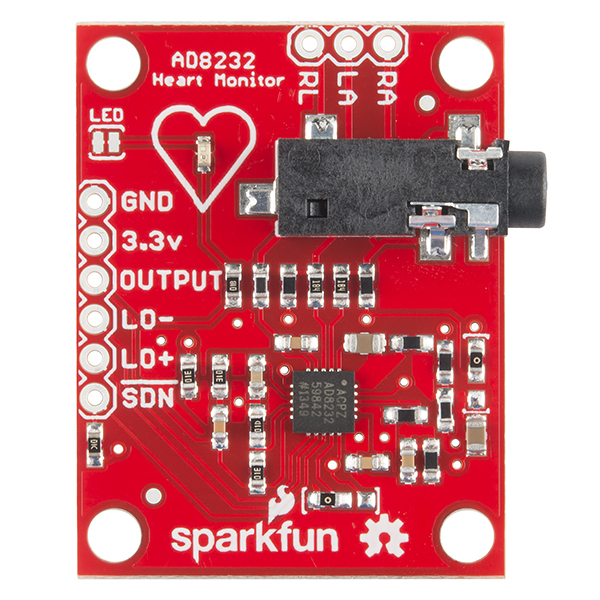
\includegraphics[width=0.3\linewidth]{ad8232sfboard.jpg}
	\caption{AD8232 Heart Rate Monitor from SparkFun Electronics \cite{ad8232}}
	\label{ad8232sfboard}
\end{figure}

\subsubsection*{Complete AD8232 ECG Sensor Setup}

Due to the absence of an analog-to-digital converter, it is necessary to use a microcontroller which is capable of this conversion and serial communication through a USB port for prototyping. As such, an Arduino Pro Mini 328 (3.3V/8MHz) was used in the development of the interface. The design of the system was sourced from SparkFun Electronics \cite{ad8232}. 

The assembly of the complete AD8232 ECG sensor requires the following components \cite{ad8232}:

\begin{enumerate}
	\item Arduino Pro Mini 328 - 3.3V/8MHz (DEV-11114)
	\item SparkFun USB Mini-B Cable - 6 foot (CAB-11301)
	\item SparkFun FTDI Basic Breakout - 3.3V (DEV-09873)
	\item Break Away Headers - Straight (PRT-00116)
	\item Sensor Cable - Electrode Pads (3 connector) (CAB-12970)
	\item Biomedical Sensor Pad (10 pack) (SEN-12969) 
	\item SparkFun Single Lead Heart Rate Monitor - AD8232 (SEN-12650) 
\end{enumerate}

These components are assembled in the pattern found in Figure \ref{ad8232sffritzing}. 

\begin{figure}[H]
	\centering
	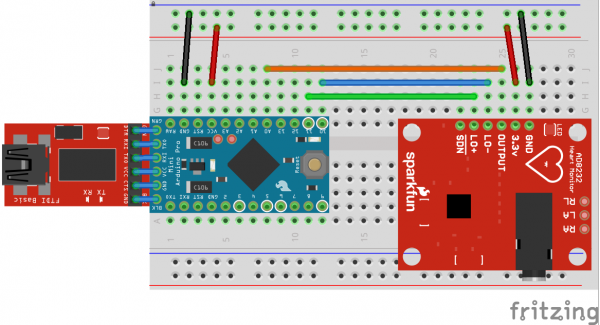
\includegraphics[width=0.5\linewidth]{ad8232fritzing.png}
	\caption{AD8232 Connection Diagram using Fritzing \cite{ad8232}}
	\label{ad8232sffritzing}
\end{figure}

In terms of the pin connections between the AD8232 and the Arduino Pro Mini, the connections are found in Table \ref{ad8232pinconfigurationtable}.

\begin{table}[H]
	\centering
	\caption{Pin Configuration for the AD8232 and the Arduino Pro Mini \cite{ad8232}}
	\label{ad8232pinconfigurationtable}
	\begin{tabular}{|l|l|l|}
		\hline
		\textbf{Board Label} & \textbf{Pin Function} & \textbf{Arduino Connection} \\ \hline
		GND                  & Ground                & GND                         \\ \hline
		3.3v                 & 3.3v Power Supply     & 3.3v                        \\ \hline
		OUTPUT               & Output Signal         & A0                          \\ \hline
		LO-                  & Leads-off Detect -    & 11                          \\ \hline
		LO+                  & Leads-off Detect +    & 10                          \\ \hline
		SDN                  & Shutdown              & Not used                    \\ \hline
	\end{tabular}
\end{table}


The complete circuit can be found in the Figure below 

\begin{figure}[H]
	\centering
	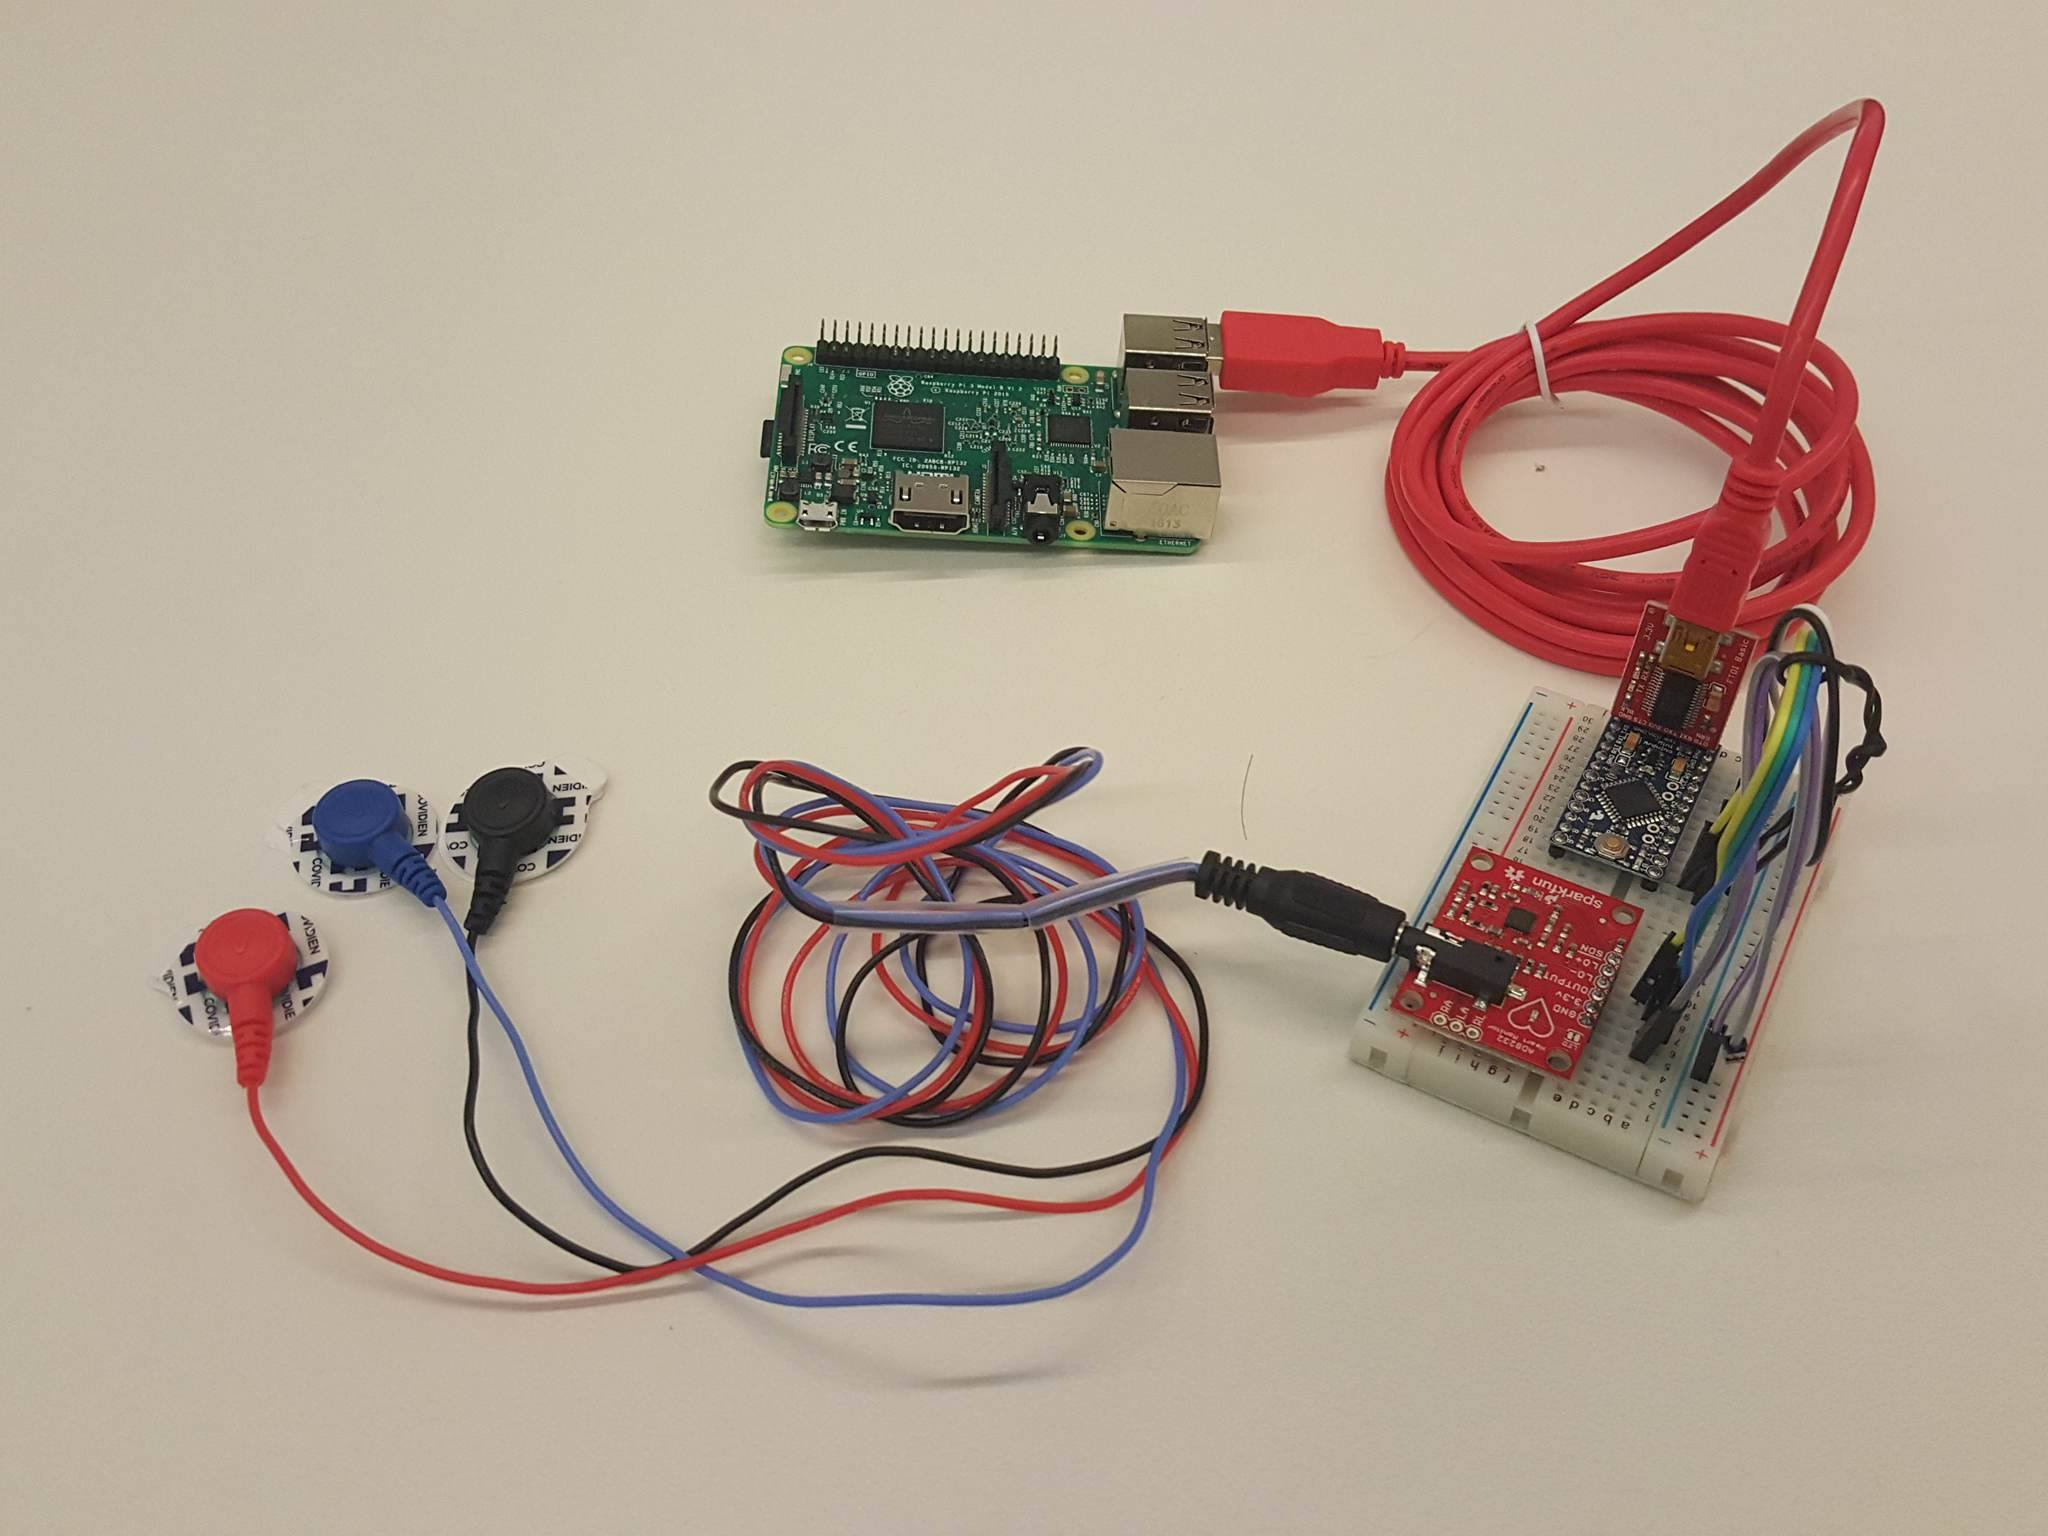
\includegraphics[width=0.6\linewidth]{ecgsetupactual.jpg}
	\caption{Actual AD8232, Arduino Pro Mini, FTDI, and Raspberry Pi Setup} %\cite{ad8232}}
	\label{ecgsetup}
\end{figure}

To circumvent the need of using a breadboard, a PCB shield for the AD8232 and the Arduino Pro Mini was designed to accomodate both breakout boards on a single board without the need for wires to connect the internal components. The PCB design can be found in Appendix \ref{ecgshieldpcb}. 



\section{EEG}

\subsection{Neurosky TGAM module}

\begin{figure}[H]
	\centering
	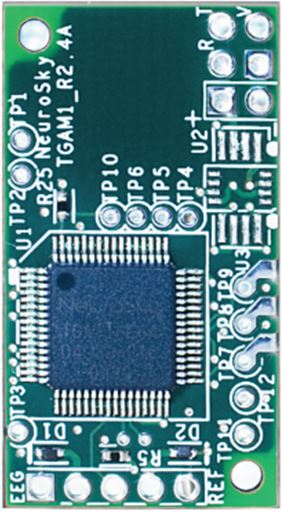
\includegraphics[width=0.25\linewidth,angle=270,origin=c]{jiahuipic2.jpg}
	\caption{Neurosky TGAM Module \cite{jiahui12}}
\end{figure}

Summary:
\begin{itemize}
\item	The TGAM module is used as a primary brainwave sensor ASIC module.
\item	Able to process and output EEG frequency spectrum, EEG single quality, raw EEG 
\item	Can be used together with simple dry electrodes
\item	Low power consumption – ideal for portable battery driven application
\end{itemize}

Features:
\begin{itemize}
\item	One EEG channel using three contact points, i.e. EEG electrode, EEG reference electrode and ground electrode
\item	Inbuilt filter system that resets when “Poor signal quality detected” for consecutive 4 seconds, or small noisy signals for 7 seconds
\item	Max power consumption at 15mA @ 3.3V
\item	Raw EEG data output at 512 bits per second
\item	Able to measure raw brainwave signal, different EEG spectrum such as Alpha, Beta, Gamma etc. 
\end{itemize}

The low power consumption as well as different EEG spectrum that provides waveform we required is the basis that this chip is selected for our proof of concept

\begin{figure}[H]
	\centering
	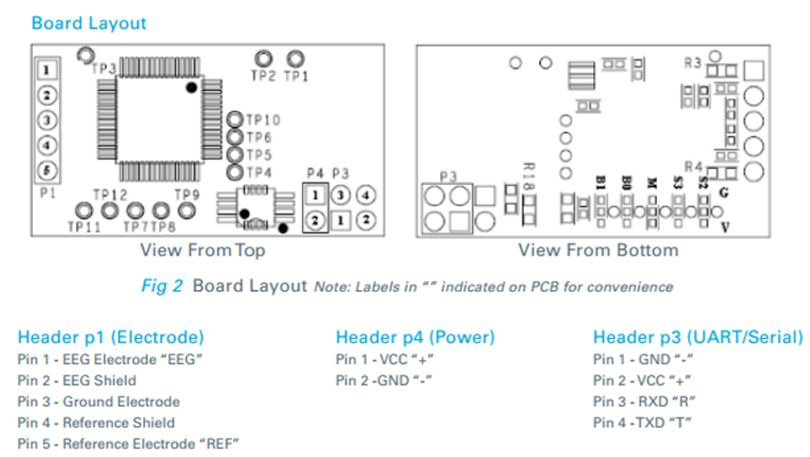
\includegraphics[width=0.7\linewidth]{jiahuipic3.jpg}
	\caption{Board Layout}
\end{figure}

During the setting up and soldering of the chip, several important steps are highlighted. First, the EEG electrode will be placed at top of the skull/forehead with applications of electrolytes gel to obtain electrical impulses for analysis. Both of the EEG and reference shield are open-ended wires that are of same length to the respective electrodes to act as an open ended reference for microchip to compute. The reference electrodes are placed at the base of the ear-lobe as it has least neurons and acts as a reference body potential to the EEG electrode. The board is powered up by a separate voltage regulator with constant 3,3V and 50mA current limit to ensure that the board will not encounter any overcurrent issue.

\begin{figure}[H]
	\centering
	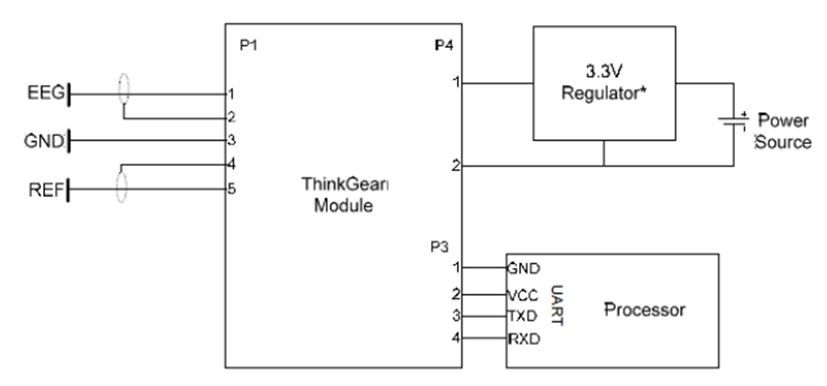
\includegraphics[width=0.7\linewidth]{jiahuipic4.jpg}
	\caption{ThinkGean Module}
\end{figure}

A 9V battery is used as the power source, and Arduino is used as an interface to capture the output data to be visualized at the console. 

\begin{figure}[H]
	\centering
	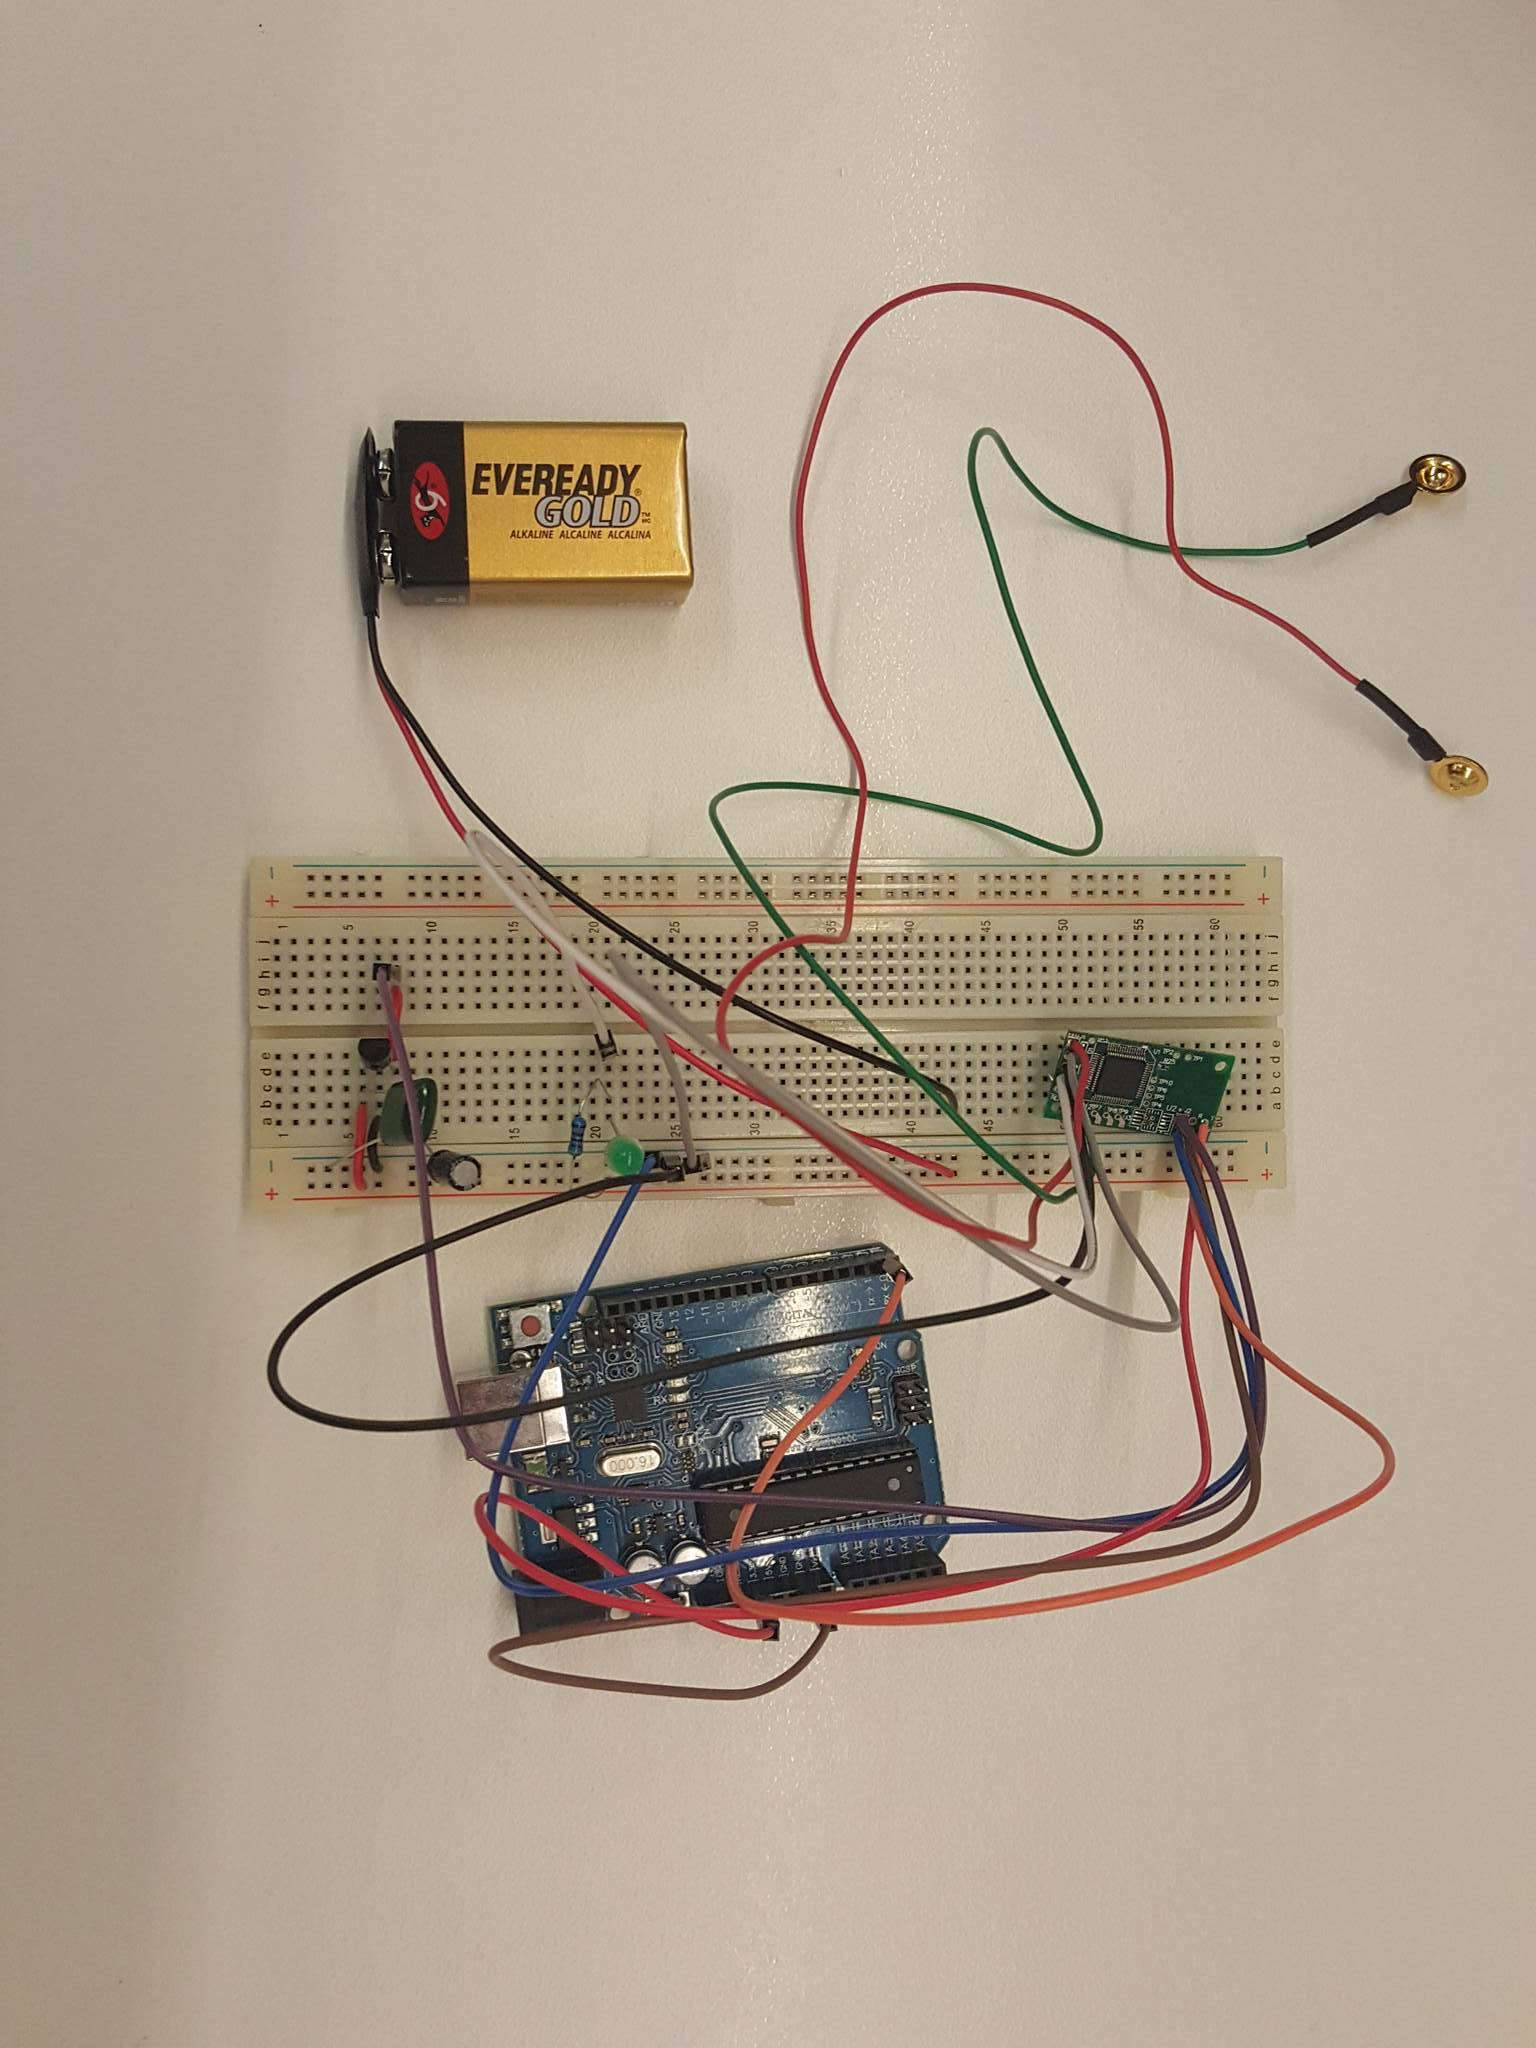
\includegraphics[width=0.4\linewidth,angle=90,origin=c]{eegsetup.jpg}
	\caption{Actual EEG Setup}
\end{figure}

\section{PPG}

When we tried to obtain the PPG waveform by directly connecting a pair of infrared transmitter and receiver with the Arduino, we were not able to visualize any valid signals. This could be due to two main reasons: 

\begin{enumerate}
	\item The photoplethysmogram signal is very small in amplitude compare with the DC offset component in the carrying signal.
	\item The pair of sensors is not working properly.	
\end{enumerate}

To eliminate the second possibility, we did some testing with the sensors along. The intensity of the infrared beams received at the receiver is proportional to the separation between the transmitter and the receiver. By moving the transmitter towards and away from the receiver, we can observe instant change of the readings. 

Hence, we come to the conclusion that the signal from our PPG sensor is very small in amplitude compare with the DC offset and the high frequency noise. Therefore, low-pass filter, high-pass filter and op-amp are used to extract the useful information from the “raw” signal from PPG sensor. 

For the Arduino we are using, it has 10-bit analog to digital convertor which maps the analog input between 0 to 5V into 1024 discrete levels between 0 and 1023. This gives the resolution around 5mV per unit. Hence, in order to obtain a clear visualization of the PPG signal, the AC component needs to be amplified to few volts in amplitude (less than supply voltage 5V). 

\subsection{Bandwidth Selection}

The frequency of the normal resting heart rate is between 1Hz to 2Hz \cite{george8}. Hence, for our Pulse Oximeter, we allow the signal between 0.5Hz to 4Hz to pass through. Extra margin is designed for special cases.

\subsection{Circuit Design}

\begin{figure}[H]
	\centering
	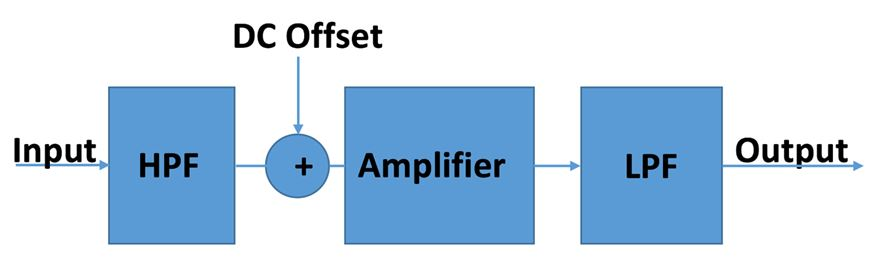
\includegraphics[width=0.7\linewidth]{georgepic3.jpg}
	\caption{Circuit Design}
\end{figure}

\begin{figure}[H]
	\centering
	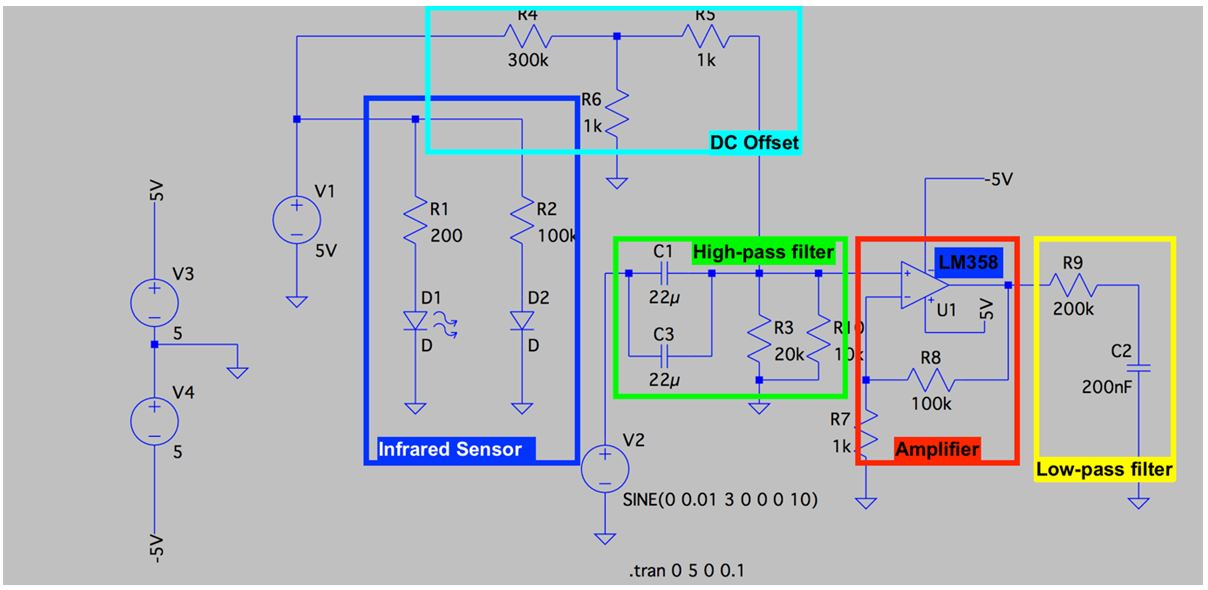
\includegraphics[width=0.9\linewidth]{georgepic4.jpg}
	\caption{Circuit Design}
\end{figure}

\subsubsection{High Pass Filter}

A RC high pass filter is designed to meet the lower bound of the bandwidth requirement.

\begin{equation}
	f_c = \frac{1}{2\pi RC}
\end{equation}

In our design, we choose $R = 6666 \Omega$ (20k and 10k in parallel) and $C = 44 \mu F$ which gives us a cut-off frequency of $0.543 Hz$.

\subsubsection{Low Pass Filter}

A RC low pass filter is designed to meet the upper bound of the bandwidth requirement.

\begin{equation}
f_c = \frac{1}{2\pi RC}
\end{equation}

In our design, we choose $R = 200k \Omega$ and $C = 200nF$ which gives us a cut-off frequency of $3.98 Hz$ which is close to $4 Hz$.

\subsubsection{Amplifier}

Since we are not able to observe any waveform from the original signal, the amplitude of the original AC component must have magnitude of few mV because the resolution of the Arduino is 5mV. If the oscillation of the original signal has few hundred mV in amplitude, the waveform would be clearly observed without any signal processing. In order to amplify the signal to the magnitude of volts, we design an amplifier with gain of 100 which gives the output in Volts. 

Another limitation is the power supply from the Arduino UNO. A normal operational amplifier requires positive and negative voltage for its supply rails. But Arduino UNO only provides positive 5V and GND. LM358 op-amp, which is used in our prototype, requires only positive voltage supply which is perfectly compatible with Arduino.

\begin{figure}[H]
	\centering
	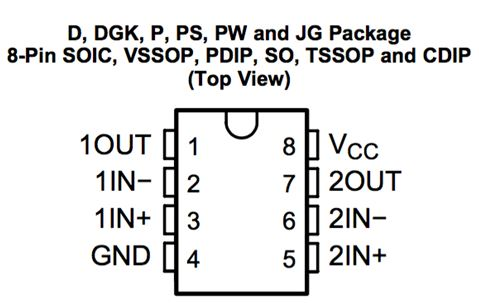
\includegraphics[width=0.3\linewidth]{georgepic5.jpg}
	\caption{LM 358 \cite{george12}}
\end{figure}

\subsubsection{Offset Voltage}

To avoid signal being saturated at 0, an offset voltage is supplied to the input signal before the amplifier. Since the Arduino UNO can detect values between 0 ~ 5V, it is reasonable to have an offset voltage of 1.5V. 

In order to achieve 1.5V offset at the output, the pre-amplified offset is set to be 1.5V/100 = 15mV, where 100 is the gain of the amplifier. Voltage divider is used to get 15 mV from a 5V source.

\subsubsection{LTSpice Simulation}

A sinusoidal input with frequency 3 Hz with peak-to-peak voltage 20 mV is used for simulation. The output is:

\begin{figure}[H]
	\centering
	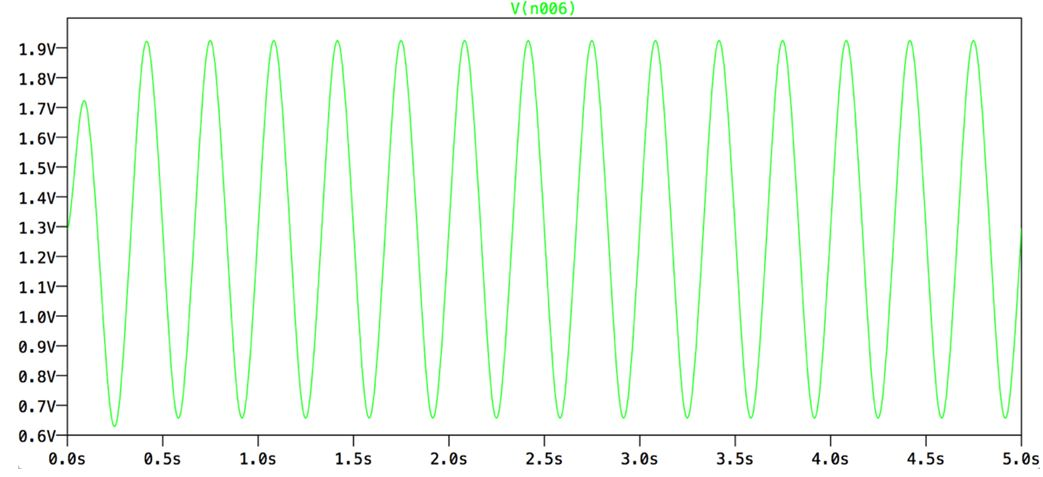
\includegraphics[width=0.7\linewidth]{georgepic7.jpg}
	\caption{Output of LTSpice Simulation}
\end{figure}

From the output plot, we are able to see the input sinusoidal signal has been amplified to roughly 1.4V peak-to-peak with 1.3V DC-offset.







\section{Blood Temperature}

\subsection{Thermistor}
\label{thermistor}

One of the methods to measure body temperature is through measuring heat conduction via direct physical contact with the patient's body. As a thermistor is a temperature-dependent resistor, the resistance of a thermistor varies with temperature. The property of thermistors therefore, are desirable in the design of a temperature sensor. 

Using an Arduino Uno for prototyping, a simple voltage divider is constructed to study the characteristics of a thermistor. The thermistor used in this project is a material type F thermistor \cite{thermistor}. The circuit in Figure \ref{temperaturefritzing1} was constructed for testing the thermistor. 

\begin{figure}[H]
	\centering
	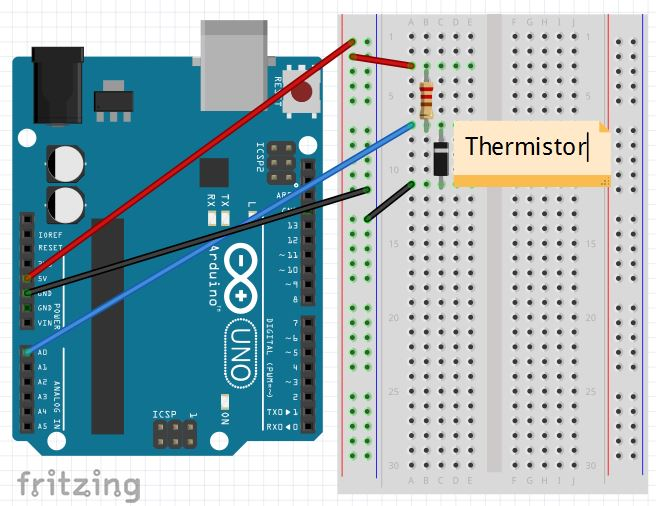
\includegraphics[width=0.5\linewidth]{temperaturefritzing1.jpg}
	\caption{Thermistor in Voltage Divider Configuration using Fritzing}
	\label{temperaturefritzing1}
\end{figure}

The datasheet of the material type F thermistor \cite{thermistor} reveals the following formulae and properties: 

\begin{figure}[H]
	\centering
	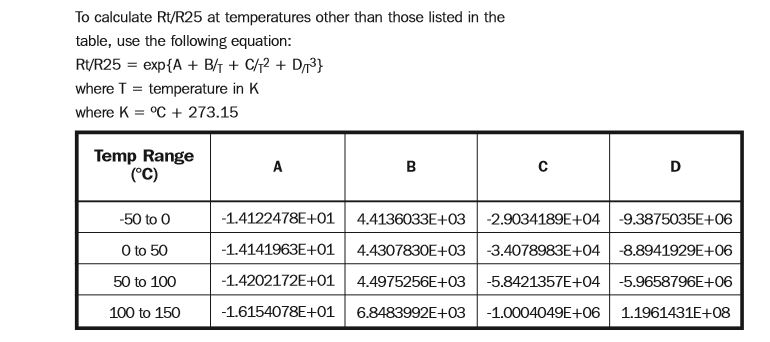
\includegraphics[width=0.8\linewidth]{thermistordatasheet2.jpg}
	\caption{Thermistor Formulae and Properties \cite{thermistor}}
	\label{thermistordatasheet2}
\end{figure}

\begin{figure}[H]
	\centering
	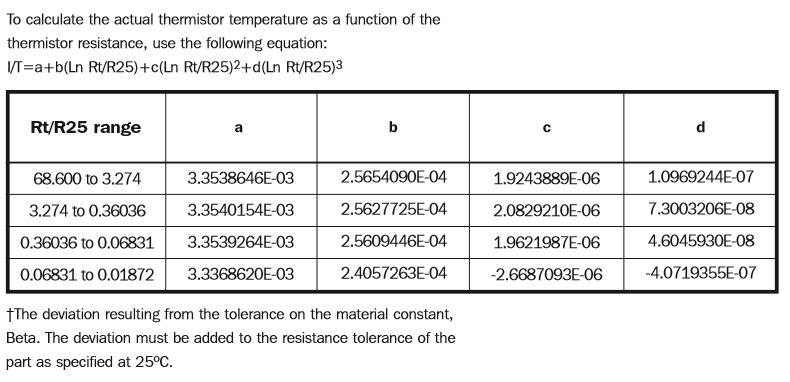
\includegraphics[width=0.8\linewidth]{thermistordatasheet3.jpg}
	\caption{Thermistor Formulae and Properties (cont.) \cite{thermistor}}
	\label{thermistordatasheet3}
\end{figure}

\begin{equation}
	\frac{Rt}{R25} = exp(A+\frac{B}{T}+\frac{C}{T^2}+\frac{D}{T^3}) 
	\label{thermistorresistance1}
\end{equation}

\begin{equation}
	\frac{1}{T} = a+b(ln\frac{Rt}{R25})+c(ln\frac{Rt}{R25})^2+d(ln\frac{Rt}{R25})^3\\
	\label{thermistorresistance2}
\end{equation}

T is the temperature in Kelvin where $K=\degree C+273.15$. 

Choosing an operating temperature range of $0\degree C$ to $50\degree C$, Equation \ref{thermistorresistance1} and \ref{thermistorresistance2} has the following parameters: 

\begin{table}[H]
	\centering
	\caption{Material Type F Thermistor Parameters for $0\degree C$ to $50\degree C$}
	\label{thermistorparameters}
	\begin{tabular}{|l|l|}
		\hline
		A = -1.4141963E+01  & a = 3.3540154E-03 \\ \hline
		B = 4.4307830E+03   & b = 2.5627725E-04 \\ \hline
		C = -3.40789983E+04 & c = 2.0829210E-06 \\ \hline
		D = -8.8941929E+06  & d = 7.3003206E-08 \\ \hline
	\end{tabular}
\end{table}

Therefore, we know that the range of $\frac{Rt}{R25}$ is between 0.36036 to 3.274. $R_{25}$ was chosen to be $10k\Omega$. This circuit was tested with the Arduino code found in Appendix \ref{arduinothermistor}. \\

It is also known that this material type F thermistor is a negative temperature coefficient (NTC) thermistor, that is, when the temperature rises, there is a decrease in resistance. 

Steps for testing Negative Temperature Coefficient (NTC) behaviour: 
\begin{enumerate}
	\item Set up circuit as in Figure \ref{temperaturefritzing1}. Attach RT between A0 and GND. Upload AnalogRead code to Arduino. 
	\item Begin Serial Monitor.
	\item Touch (for a few seconds) and release thermistor with bare fingers. 
	\item Once the value stabilises, insert data into Microsoft Excel for plotting. 
\end{enumerate}

\begin{figure}[H]
	\centering
	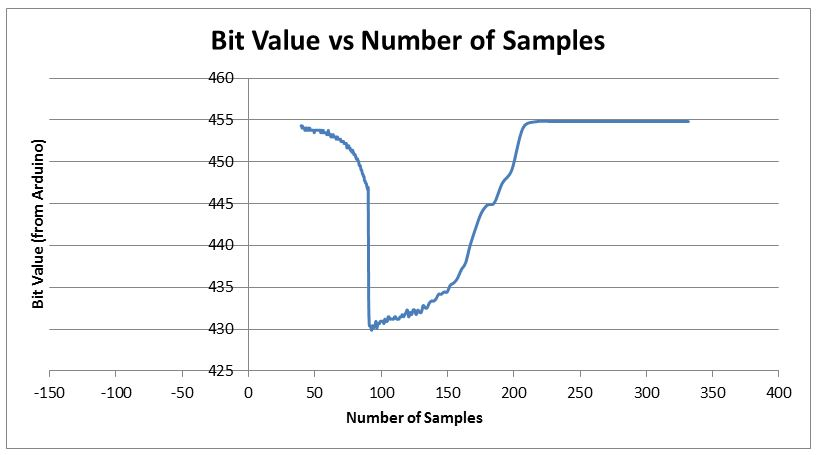
\includegraphics[width=0.8\linewidth]{thermistor1.jpg}
	\caption{Bit Value vs Number of Samples}
	\label{bitvaluevssamples}
\end{figure}

From Figure \ref{bitvaluevssamples}, when the thermistor is touched, the sensorValue decreases. This is corresponds to a decrease in RT when the temperature increases. The thermistor therefore is consistent with a NTC thermistor. 

A simple voltage division describes the above behaviour: 

\begin{equation}
	\frac{RT}{R25}=\frac{sV}{1023-sV}
	\label{thermistorresistance3}
\end{equation}

The bit range of an Arduino Uno is 1024 bits, meaning that there are 1024 bits $(0\sim 1023)$ which describe the input into A0 as there are $2^{10}$ different voltage levels for the analog input of an Arduino Uno. sV represents the detected sensorValue. 


\subsubsection{Analysis of Nonlinearity between Thermistor Resistance and Bit Value of the Arduino}

The following graph is obtained by plotting the relationship between temperature and bit value using Equation \ref{thermistorresistance1} and \ref{thermistorresistance3}, by iterating through all possible values of the sensorValue within the bit range.

\begin{figure}[H]
	\centering
	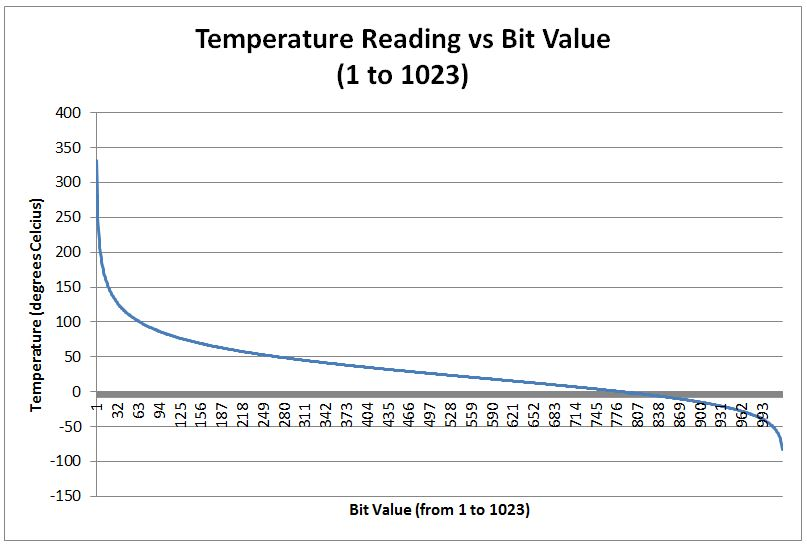
\includegraphics[width=0.7\linewidth]{thermistor2.jpg}
	\caption{Temperature Reading vs Bit Value}
	\label{temperaturevsbitvalue}
\end{figure}

The graph shown in Figure \ref{temperaturevsbitvalue} indicates that the relationship between the thermistor resistance and the bit value registered is nonlinear. However, we are only interested in the values between the range of $5\degree C$ to $45\degree C$ (narrower for better accuracy). Plotting the same graph for this specified range yields Figure \ref{temperaturevsbitvalue5-45} 

\begin{figure}[H]
	\centering
	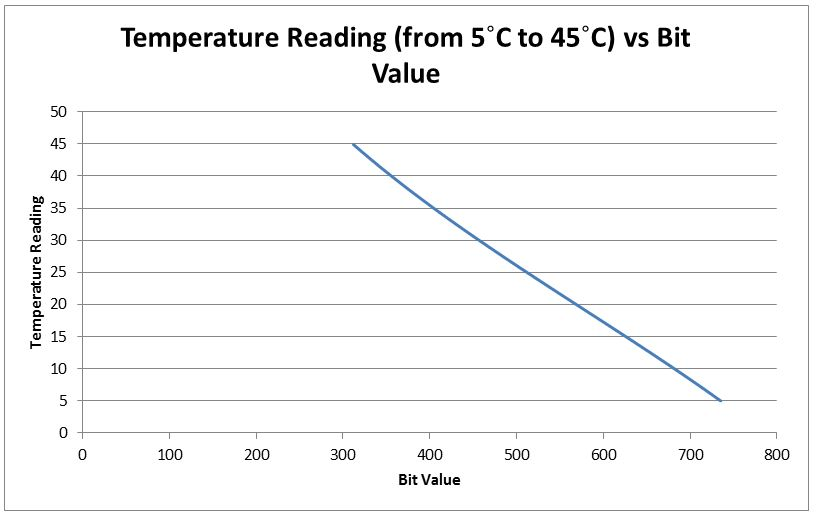
\includegraphics[width=0.7\linewidth]{thermistor3.jpg}
	\caption{Temperature Reading ($5\degree C$ to $45\degree C$) vs Bit Value}
	\label{temperaturevsbitvalue5-45}
\end{figure}

By keeping within the range of $5\degree C$ to $45\degree C$, the relationship between the thermistor resistance (given by the temperature) and the bit value of the Arduino is approximately linear.

Within $5\degree C$ to $45\degree C$, the bit values that represent this temperature range are between 312 and 735. Roughly 424 bits are used to represent $5\degree C$ to $45\degree C$ in the analog-to-digital converter of the Arduino Uno. 

\subsubsection{Sensitivity Analysis of Material Type F Thermistor}

The derivative of Equation \ref{thermistorresistance1} is: 
\begin{equation}
	\frac{d(RT/R25)}{dt}=-\left (\frac{B}{T^2}+\frac{2C}{T^3}+\frac{3D}{T^4} \right ) exp(A+\frac{B}{T}+\frac{C}{T^2}+\frac{D}{T^3}) 
	\label{thermistorderivative}
\end{equation}

By plotting Equation \ref{thermistorderivative} (the time derivative of RT/R25) for the temperature range between 275K and 350K, we obtain Figure \ref{dRTR25dttemperature}. 

\begin{figure}[H]
	\centering
	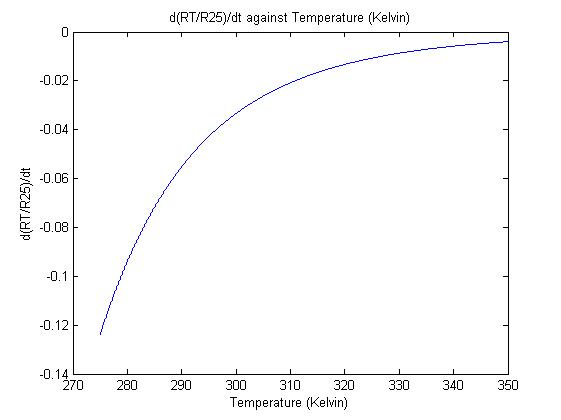
\includegraphics[width=0.65\linewidth]{thermistor5.jpg}
	\caption{$\frac{d(RT/R25)}{dt}$ against Temperature (Kelvin)}
	\label{dRTR25dttemperature}
\end{figure}

Figure \ref{dRTR25dttemperature} shows that as temperature increases (270K to 350K), the rate of change of RT/R25 decreases that is, as $\Delta T$ increases, $\Delta R$ decreases.  A change in temperature at lower temperatures gives a bigger change in resistance than a change in temperature at higher temperatures. Hence, the sensitivity of the thermistor decreases as temperature increases. 

\subsubsection{Self-Heating of Negative Temperature Coefficient (NTC) Thermistor}

Due to the nature of negative temperature coefficient (NTC) thermistors, it can be deduced that the higher the temperature, the lower the resistance of the thermistor. By having a lower resistance with the same voltage across the component, the current through the component increases due to the relation in Equation \ref{vir}. An increase in current always translates to more heat being dissipated across a resistor, thereby increasing its temperature. As such, there is a positive feedback mechanism for NTC type thermistors, leading to the problem of self-heating. This affects the accuracy of devices which use thermistors as voltage dividers. Hence, the thermistor configuration used above in Figure \ref{temperaturefritzing1} is only suitable for testing the properties of the material type F thermistor but not for actual temperature measurement.  

\begin{equation}
 V=IR
 \label{vir}
\end{equation} 

\subsection{Thermistor in Phase Shift Oscillator (PSO) Configuration}

To circumvent the issue of self-heating of NTC thermistors in Section \ref{thermistor} above, it is necessary to reduce the amount of current flowing through the component. 

From the voltage division perspective, temperature is resistance-dependent. However, it is possible to make temperature dependent on frequency by implementing thermistor coupled with a phase shift oscillator.  

The phase shift oscillator (PSO) is an oscillator with a resistor-capacitor network, leading to regenerative feedback which produces a sine wave output signal \cite{psotutorial}. This regenerative feedback is due to the charge storage capacity of the capacitor \cite{psotutorial}. 

\begin{figure}[H]
	\centering
	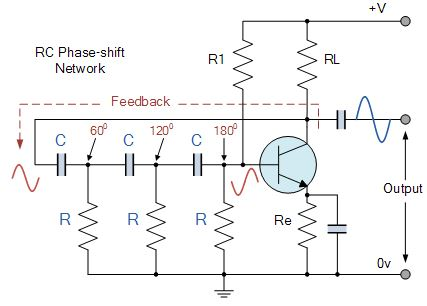
\includegraphics[width=0.6\linewidth]{psowebsite.jpg}
	\caption{Basic RC Oscillator Circuit (Phase Shift Oscillator) \cite{psotutorial}}
	\label{psowebsite}
\end{figure}

One of the properties of the phase shift oscillator is the change in frequency when any of the values of the resistances in the phase shift network is adjusted. This leads to the dependence of the output frequency on the resistance.  

By replacing one of the resistors with a thermistor, it is then possible to keep the current relatively small across the thermistor while still measuring the change in temperature based on the change in frequency. Hence, using a thermistor coupled with phase shift oscillator helps to mitigate the issue of self-heating in the thermistor.  

The frequency of the oscillations of the phase shift oscillator is governed by the following formula \cite{psotutorial}:
\begin{equation}
	f_r = \frac{1}{2 \pi RC \sqrt{2N}}
	\label{frequencyoutput}
\end{equation} 

Where:  \\
$f_r$ is the Output Frequency in Hz \\
$R$ is the Resistance in $\Omega$ \\
$C$ is the Capacitance in $F$ \\
$N$ is the Number of RC stages ($N=3$) \\

Based on the phase shift oscillator design by Dr. Peter Farrell from the University of Melbourne, the following circuit was simulated in LTSpice \cite{peterfarrell}: 

\begin{figure}[H]
	\centering
	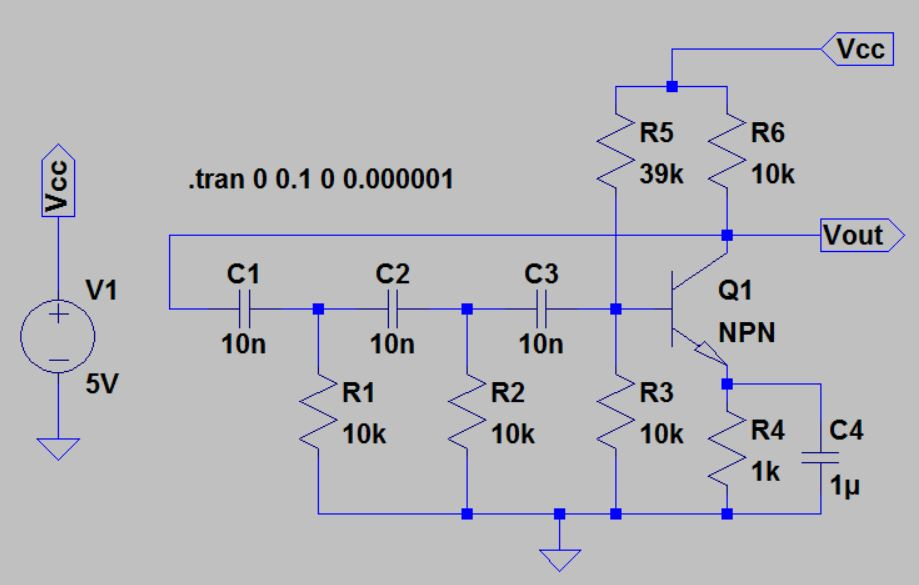
\includegraphics[width=0.7\linewidth]{psoltspice.jpg}
	\caption{Phase Shift Oscillator Circuit in LTSpice \cite{peterfarrell}}
	\label{psoltspice}
\end{figure}
